\documentclass{beamer}

\usetheme{Copenhagen}
\usepackage[utf8]{inputenc}
\usepackage{graphics}

% Slayt basliklarinda kullanilan font boyutu
\setbeamerfont{frametitle}{size=\normalsize}

\title{Kenar Algılama}
\author{Nurettin Şenyer}
\date{19 Mayıs, 2011}
\institute[2011]{19/x}

\begin{document}

\frame{\titlepage}

\frame {
	\frametitle{Çapraz İlinti (cross-correlation)}

	$F$ resmini ve $H$ kernel işlevi ($2k+1 x 2k+1$) olsun, bu durumda $G$,

	$G[i,j] = \sum_{u=-k}^{k} \sum_{v=-k}^{k} H[u,v] F[i+u, j+v]$

	bu çapraz ilintidir

	$G = H \times F$
}

\frame {
	\frametitle{Katlama}

	çapraz-ilintiyle aynı fakat kernel işlevi her iki eksende yansıtılmıştır,

	$G[i,j] = \sum_{u=-k}^{k} \sum_{v=-k}^{k} H[u,v] F[i-u, j-v]$

	bu katlama işlemidir,

	$G = H * F$
}

\frame {
	\frametitle {ilinti X katlama}

	\begin{columns}
		\column{0.5\textwidth}
			çapraz ilinti

			\begin{itemize}
				\item yer değiştime yoktur

				\item dağılma

				$F \times (G \times H) = (F \times G) \times H$

				\item birimsellik: yoktur
			\end{itemize}

		\column{0.5\textwidth}
			katlama

			\begin{itemize}
				\item yer değiştirme: $F * G = G * F$

				\item dağılma

				$F * (G * H) = (F * G) * H$

				\item birimsellik

				$I * \delta = I$
			\end{itemize}

	\end{columns}
}

\frame {
	\framtitle {kenar algılama}

	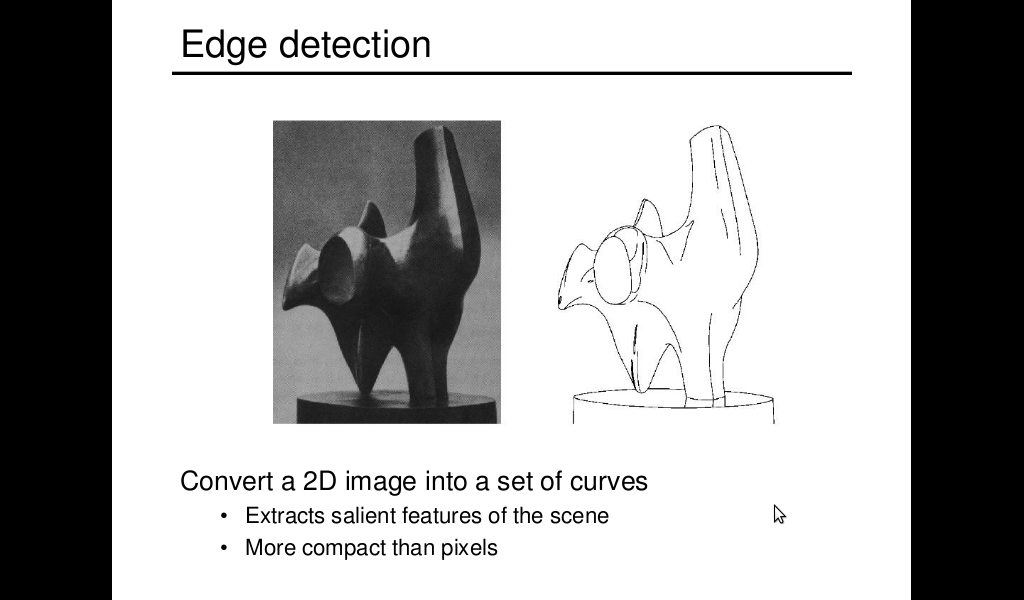
\includegraphics[width=0.2\textwidth]{img/fig06-edge.png}

	Resmi 2B resmi, eğriler kümesine dönüştür

	\begin{itemize}
		\item sahneden öznitelikleri çıkart

		\item pikselleri daha kompakt ifade et
	\end{itemize}
}

\frame {
	\frametitle {kenar}

	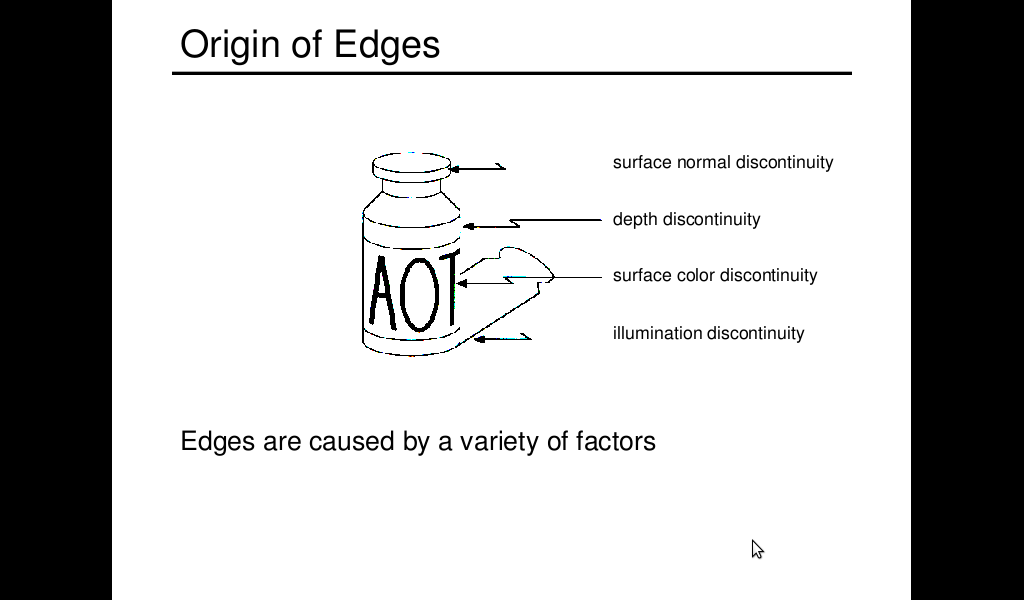
\includegraphics[width=0.2\textwidth]{img/fig07-kenar.png}

	Kenar, çok sayıda farklı kaynaktan meydana gelir
}

\frame {
	\frametitle {kenar algılama}

	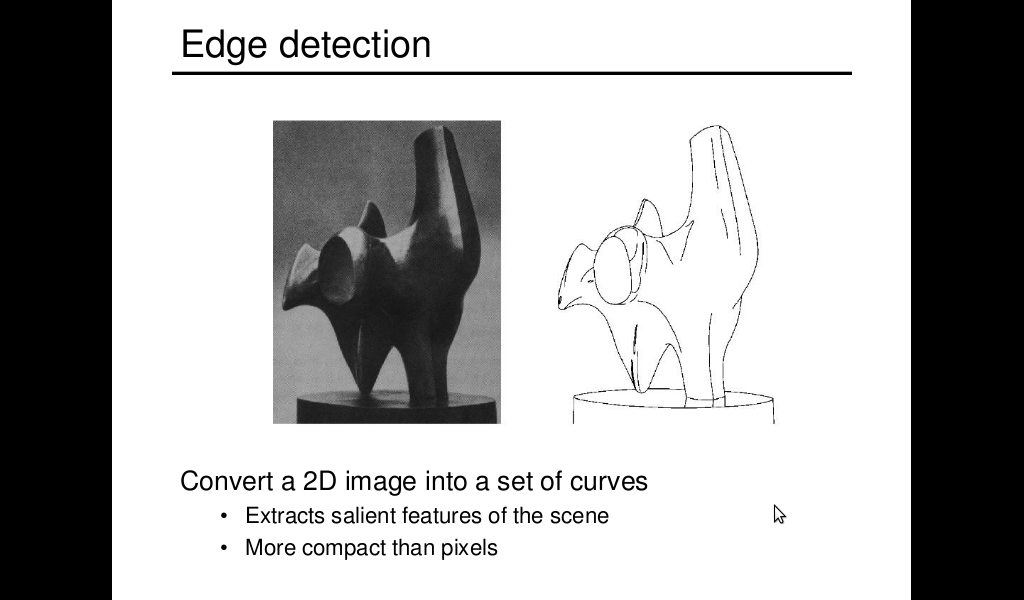
\includegraphics[width=0.2\textwidth]{img/fig06-edge.png}

	piksellerin bir kenara ait olup-olmadığını nasıl söyleyebiliriz?
}

\frame {
	\frametitle {resim gradyanı}

	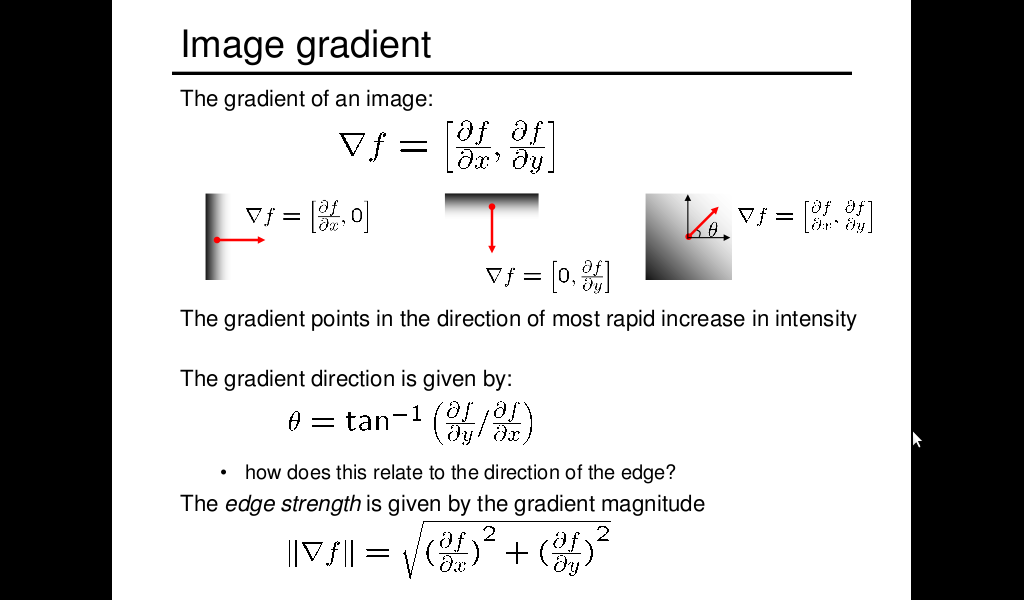
\includegraphics[width=0.2\textwidth]{img/fig10-grad.png}

	gradyan: parlaklığın en hızlı değiştiği yöndür

	gradyan yönü: $\theta = atan(df/dy / df/dx)$

	genliği=kenar gücü: $|Df| = \sqrt{(df/dx)^2 + (df/dy)^2}$
}

\frame {
	\frametitle {ayrık gradyan}

	ayrık - $F[x,y]$ için türev nasıl?

	$dF/dx = lim (h->0) \frac{F(x+h,y) - F(x,y)}{h}$

	sonlu farklar: $dF/dx ~ F[x+1,y] - F[x,y]$

	çapraz ilintiyle gerçekleme: $H = [0 0 0; 1/2 0 -1/2; 0 0 0]$
}

\frame {
	\frametitle {sobel}

	en yaygın kullanılanlarındandır: $S_y = 1/8 * [-1 -2 -1; 0 0 0; 1 2 1]$ ve $S_x =
	S_y'$
}

\frame {
	\frametitle {gürültü}

	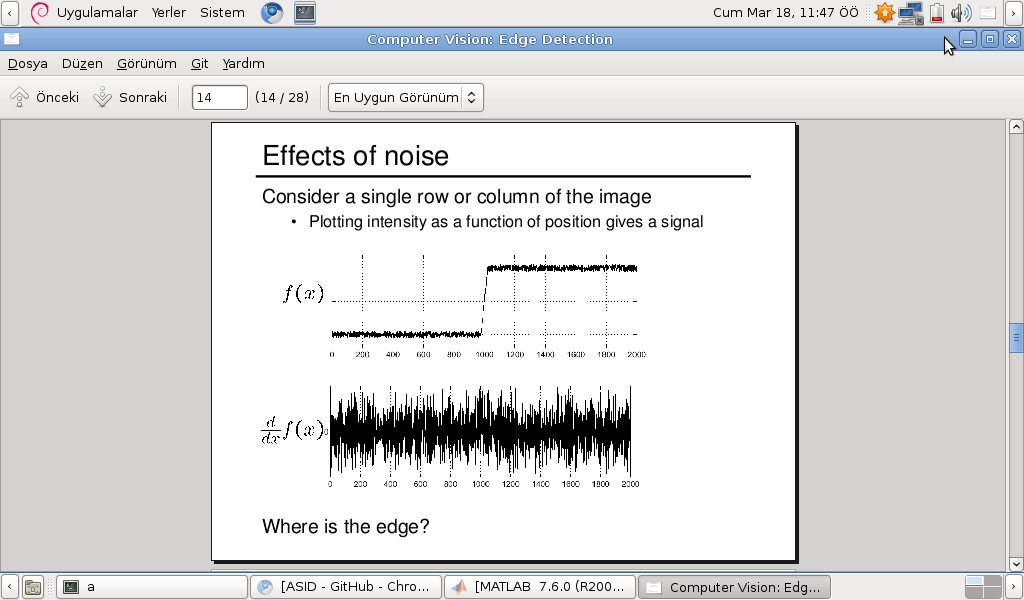
\includegraphics[width=0.2\textwidth]{img/fig14-gurultu.png}

	türevden kenarı bulmak zor!
}

\frame {
	\frametitle {çözüm: yumuşatma}

	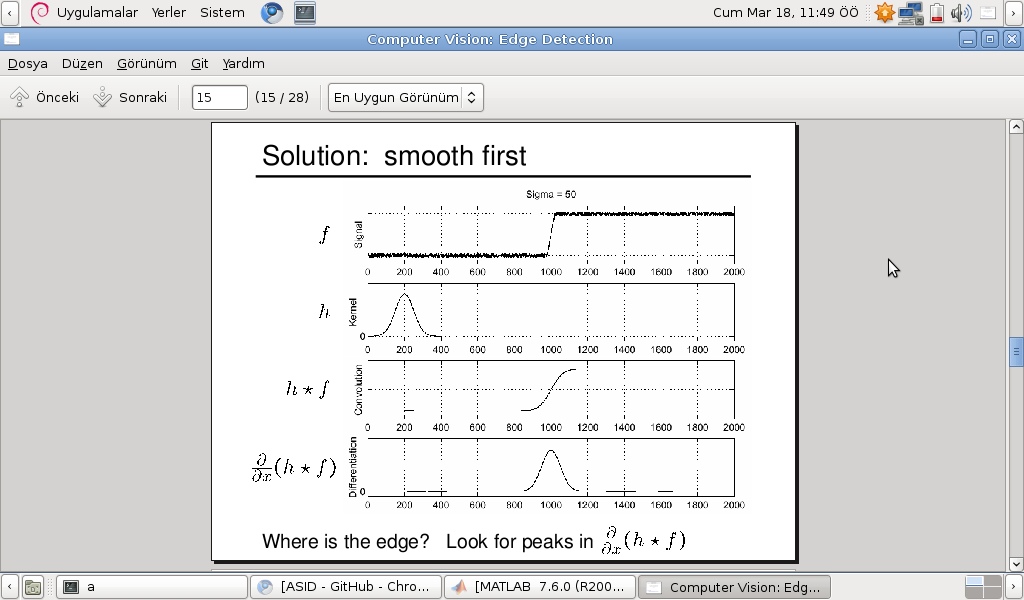
\includegraphics[width=0.2\textwidth]{img/fig15-yumus.png}
}

\end{document}
